\documentclass{TechReport}
 \usepackage{listings}
 \usepackage{courier}
%\definecolor{mauve}{rgb}{0.88, 0.69, 1.0}
\definecolor{burgundy}{rgb}{0.5, 0.0, 0.13}
\definecolor{dkgreen}{rgb}{0.0, 0.5, 0.0}
\definecolor{cardinal}{rgb}{0.77, 0.12, 0.23}
\lstset{ %
  language=R,                     % the language of the code
  basicstyle=\small\ttfamily,       % the size of the fonts that are used for the code
  numbers=left,                   % where to put the line-numbers
  numberstyle=\tiny\color{gray},  % the style that is used for the line-numbers
  stepnumber=0,                   % the step between two line-numbers. If it's 1, each line
                                  % will be numbered
 numbersep=5pt,                  % how far the line-numbers are from the code
  backgroundcolor=\color{white},  % choose the background color. You must add \usepackage{color}
  showspaces=false,               % show spaces adding particular underscores
  showstringspaces=false,         % underline spaces within strings
  showtabs=false,                 % show tabs within strings adding particular underscores
  frame=none,                   % adds a frame around the code
 rulecolor=\color{black},        % if not set, the frame-color may be changed on line-breaks within not-black text (e.g. commens (green here))
  tabsize=2,                      % sets default tabsize to 2 spaces
  captionpos=b,                   % sets the caption-position to bottom
  breaklines=true,                % sets automatic line breaking
  breakatwhitespace=false,        % sets if automatic breaks should only happen at whitespace
  title=\lstname,                 % show the filename of files included with \lstinputlisting;
                                  % also try caption instead of title
  keywordstyle=\color{blue},      % keyword style
  commentstyle=\color{dkgreen},   % comment style
  stringstyle=\color{cardinal},      % string literal style
  escapeinside={\%*}{*)},         % if you want to add a comment within your code
  morekeywords={*,...}            % if you want to add more keywords to the set
} 

\usepackage{color}
\usepackage{subfigure}
\usepackage{url}
\newcommand{\urlwofont}[1]
{
\urlstyle{same}\url{#1}
}
%--------------
\lstdefinestyle{base}{
  moredelim=**[is][\color{blue}]{@}{@}
}
%\setkomafont{sectioning}{\bfseries}
\usepackage[numbib]{tocbibind}
\renewcommand{\listoffigures}{\begingroup
\tocsection
\tocfile{\listfigurename}{lof}
\endgroup}
\usepackage[english]{babel}
\usepackage[bottom,hang]{footmisc}
\setlength{\footnotemargin}{0pt}



\title{EasyTCGA:\\ An R package for easy batch downloading of TCGA data from FireBrowse}
\author{Viktoria Kliewer \& Sangkyun Lee}
\date{09/2016}        %Serial Number/Year

\begin{document}
\makesfbtitlepage

\section{Introduction}
Many organizations deal with the investigation of cancer including the National
Institutes of Health, USA.
% the National Cancer Institute (NCI) Center for Cancer
Genomics(CCG)\footnote{\url{http://www.cancer.gov/about-nci/organization/ccg}}. 
The Cancer Genome Atlas (TCGA)\footnote{\url{http://cancergenome.nih.gov/}} is an
establishment of the
National Cancer Institute (NCI) and the National Human Genome Research Institute
(NHGRI)
that has created maps of the key genomic changes in more than 30 cancer types. The
aim of TCGA is the improvement
of the effectiveness to diagnose, treat and to guard against cancer through genome
analysis. TCGA provides a
publically available dataset.\\
The Broad Institute TCGA GDAC
Firehose\footnote{\url{https://gdac.broadinstitute.org/#}} arranges this
data set that can be loaded directly with use of
FireBrowse\footnote{\url{http://firebrowse.org/}}. FireBrowse allows
simple and smart download and study TCGA data and TCGA analyses. The data is
downloaded as zip files.\\
Mario Deng created an R client called \texttt{\em FirebrowseR} with the objective of
getting the TCGA data from FireBrowse conveniently.
The size of record sets to download is limited. \texttt{\em EasyTCGA} is an R
package providing easy batch downloading of particular
TCGA data from FireBrowse using \texttt{\em FirebrowseR}. The key advantage of
EasyTCGA is the downloading of the whole available
data set you are interested in at once as a single data frame. \\
The focus of this technical report is on the presentation of the R package
\texttt{\em EasyTCGA}. That's why all specific expressions and variables 
like biological data and the like won't be explained. You get all relevant
background informations on the given URL's.\\
\texttt{\em EasyTGCA} can download clinical data, sample-level log2 miRSeq and
mRNASeq expression values, selected columns
from the MAF (Mutation Annotation File) generated by MutSig and significantly
mutated genes, as scored by MutSig.\\

\subsection{Installation}
The package is available at
GitHub\footnote{\url{https://github.com/sanglee/EasyTCGA}}. Type the following
command in R console:
\begin{lstlisting}[style=base]
@> devtools::install_github("sanglee/EasyTCGA")@
\end{lstlisting}
Before downloading data with \texttt{\em FirebroweR} and \texttt{\em EasyTCGA} it is
recommandable to check if the data to query is available 
on FireBrowse\footnotemark[4].\\

\section{Functionality of EasyTCGA}
This section gives an overview of the R package \texttt{\em EasyTCGA} to acquaint
the user with this package and to get started to use it.\\
We will present the functions, some sensible steps and codes and the respective
outputs. You find the detailed description in the
documentation of the package.\\
First, load the \texttt{\em EasyTCGA} package:
\begin{lstlisting}[style=base]
@> load(EasyTCGA)@
\end{lstlisting}
All packages required for this package, including how to install \texttt{\em
FirebrowseR}, are loaded automatically.\\
Note that entries in the downloaded data frame can be "NA", "None", empty or the output is even
"NULL" if the data for your query is incomplete or there isn't any.\\

\subsection{Clinical data}
First, you should deal with clinical data, see the file $dn\_clinical.R$ of GitHub.
Especially this data provides all available cancer types, called "cohorts", 
and the TCGA  "patient barcodes"  of single, multiple or all cancer types. These
parameters, namely cohorts and patient barcodes, are the most
important input arguments for the functions of \texttt{\em EasyTCGA}. \\
The command
\begin{lstlisting}[style=base]
@> cohorts = dn_cohorts()
> cohorts
 [1] "ACC"  "BLCA" "BRCA"   "CESC" "CHOL" "COAD"  "COADREAD" "DLBC"  
    "ESCA"    
[10] "FPPP" "GBM"  "GBMLGG" "HNSC" "KICH" "KIPAN" "KIRC"     "KIRP"  "LAML"    
[19] "LGG"  "LIHC" "LUAD"   "LUSC" "MESO" "OV"    "PAAD"     "PCPG"  "PRAD"    
[28] "READ" "SARC" "SKCM"   "STAD" "STES" "TGCT"  "THCA"     "THYM"  "UCEC"    
[37] "UCS"  "UVM"   @
\end{lstlisting}
outputs a character vector containing all TCGA cohort abbreviations which are
relevant for the algorithms.\\
Use the function $dn\_clinical\_one$ to download all available clinical data of a
single cohort. Specify the input argument {\tt cohort}, e.g. BRCA 
(Breast invasive carcinoma):  
\begin{lstlisting}[style=base]
@> cohort = "BRCA"
> brca.clinical = dn_clinical_one(cohort)@
\end{lstlisting}
At the present {\tt brca.clinical} is a data frame of 1097 observations (patients)
and 111 variables, these are clinical data elements (CDEs) like 
gender, age, race, duration of the illness and biological data. All available CDEs
can be downloaded as a character vector using the 
function $Metadata.ClinicalNames$ of \texttt{\em FirebrowseR}:
\begin{lstlisting}[style=base]
@> clinical.names = Metadata.ClinicalNames(format = "csv")@
\end{lstlisting}
An extract of the data frame {\tt brca.clinical} querring information about the CDEs
{\tt tcga\_participant\_barcode, days\_to\_birth and bcra\_canonical\_reason}:
\begin{lstlisting}[style=base]
@> brca.clinical[1:3, c("tcga_participant_barcode", "days_to_bi-
rth", "bcr_canonical_reason")]
   tcga_participant_barcode  days_to_birth  bcr_canonical_reason
1             TCGA-3C-AAAU         -20211                  <NA>
2             TCGA-3C-AALI         -18538                  <NA>
3             TCGA-3C-AALJ         -22848                  <NA>@
\end{lstlisting}
\ \\
There is also a possibility of downloading clinical data of multiple cohorts or all
available clinical data as a single data frame
applying the function $dn\_clinical$. The command
\begin{lstlisting}[style=base]
@> all.clinical = dn_clinical(cohorts)@
\end{lstlisting}
returns all available clinical data.\\
To extract TCGA patient barcodes as a character vector from downloaded clinical
data, as {\tt brca.clinical} or {\tt all.clinical}, use
\begin{lstlisting}[style=base]
@> brca.barcodes = patient_barcodes(brca.clinical)
> all.barcodes = patient_barcodes(all.clinical)@
\end{lstlisting}

\subsection{Sample-level log2 miRSeq and mRNASeq data}
This section presents the approach of the files $dn\_miRNA.R$ of GitHub, containing
the functions $dn\_miRSeq$ and $dn\_miRSeq\_cohort$, and $dn\_mRNA.R$, 
containing the functions $dn\_mRNASeq$ and $dn\_mRNASeq\_cohort$. All data frames of
sample-level log2 miRSeq data provide information about the 
variables {\tt tcga\_participant\_barcode}, {\tt mir} (a micro ribonucleic acid,
miRNA ), {\tt expression\_log2}, {\tt tool}, {\tt cohort}, {\tt sample\_type} and
{\tt date}. The variables of sample-level log2 
mRNASeq data are {\tt tcga\_participant\_barcode, gene} (messenger RNA, mRNA), {\tt
expression\_log2}, {\tt z.score}, {\tt cohort}, {\tt sample\_type}, 
{\tt protocol} and {\tt geneID}.\\
The function $Metadata.SampleTypes$ of \texttt{\em FirebrowseR} returns all TCGA
sample type codes, both numeric and symbolic.
\begin{lstlisting}[style=base]
@> sample.types = Metadata.SampleTypes(format = "csv")@
 \end{lstlisting}
We download data of all sample types available.\\
There are the R files $miRNA\_ID.R$ and $mRNA\_ID.R$ which provide all available
mirs and genes for these algorithms. The ID's are as follows:
\begin{lstlisting}[style=base]
@> length(miRNA_ID)
[1] 2588
>  miRNA_ID[1:5]  # provided by the package
[1] "hsa-let-7a-2-3p" "hsa-let-7a-3p" "hsa-let-7a-5p" 
[4] "hsa-let-7b-3p"   "hsa-let-7b-5p"         
> length(mRNA_ID)
[1] 20501
> mRNA_ID[1:5]  # provided by the package
[1] "A1BG"  "A1CF"  "A2BP1" "A2LD1" "A2M"  @
\end{lstlisting}
The function $dn\_miRSeq$ with input parameters  {\tt tcga\_participant\_barcode},
{\tt mir}, {\tt coho-}\\ {\tt rt}, {\tt page.Size} and {\tt sort\_by} is intended to download 
rather small and diverse data sets, e.g. specifying just some mirs, cohorts and
barcodes.
\begin{lstlisting}[style=base]
@> mir = miRNA_ID[1:10]
> cohort = "BLCA"
> tcga_participant_barcode = " TCGA-ZF-AA53 "  
  # a TCGA patient barcode from BLCA
> page.Size = 250 
> sort_by =  "tcga_participant_barcode"
> obj = dn_miRSeq(mir,cohort,tcga_participant_barcode,sort_by, 
page.Size)@
\end{lstlisting}
{\tt obj} is a data frame with 5 observations of 7 variables.
\begin{lstlisting}[style=base]
@> obj
   tcga_participant_barcode            mir  expression_log2
1             TCGA-ZF-AA53   hsa-let-7b-3p        4.2048666
2             TCGA-ZF-AA53   hsa-let-7b-5p       13.4371320
3             TCGA-ZF-AA53 hsa-let-7a-2-3p        0.7719075
4             TCGA-ZF-AA53   hsa-let-7a-3p        4.7987074
5             TCGA-ZF-AA53   hsa-let-7a-5p       14.3184761

                      tool cohort sample_type                  date         
1 miRseq_Mature_Preprocess   BLCA          TP   2016-01-28 00:00:00
2 miRseq_Mature_Preprocess   BLCA          TP   2016-01-28 00:00:00
3 miRseq_Mature_Preprocess   BLCA          TP   2016-01-28 00:00:00
4 miRseq_Mature_Preprocess   BLCA          TP   2016-01-28 00:00:00
5 miRseq_Mature_Preprocess   BLCA          TP   2016-01-28 00:00:00
\end{lstlisting}
In contrast, $dn\_miRSeq\_cohort$ with input parameters {\tt cohort} and {\tt
page.Size} supplies the download of all available sample-level log2 miRSeq
expression 
values of one cohort as a single data frame. 
Remark that these data sets are quite big, so especially for cohorts with a large
number of patients the download will take much time. The command
\begin{lstlisting}[style=base]
@> cohort = "TGCT"
> page_size = 2000
> tgct.miRSeq = dn_miRSeq_cohort(cohort, page.Size)@
\end{lstlisting}
outputs a data frame of all available sample-level log2 miRSeq expression values of
the cohort TGCT. \\
The functions of $dn\_miRNA.R$ and $dn\_mRNA.R$ are constructed analogously.
Therefore we limit the presentation to the download of sample-level 
log2 miRSeq expression values. 

\subsubsection{Reshape}
The log2 expression values, variable {\tt expression\_log2}, corresponding to a
patient barcode and a mir is the most important information provided by 
the sample-level log2 miRSeq and mRNASeq data. This consideration resulted in the
development of reshaping algorithms for these data types. \\
The file $reshape.R$ contains the functions $reshape.miRSeq$ and $reshape.mRNASeq$
used to reshape sample-level log2 miRSeq and mRNASeq 
expression values of the sample type TP. I.e., first use the functions from 
$dn\_miRNA.R$ or $dn\_mRNA.R$ to download the input parameter {\tt data}
of $reshape.miRSeq$ or $reshape.mRNASeq$ before reshaping. \\
The function $reshape.miRSeq$ with the input parameter {\tt data} return a
$nxp$-matrix $M = (m_{ij})_{i=1,..,n, j=1,...,p}$, \ $n$ = number of patients and 
$p$ = number of mirs, rownames of the matrix correspond to the patients, colnames
correspond to the mirs,  so the following applies
\begin{center}
$m_{ij}= (expression\_log2)_{ij}$\ \  where \\
$data\$tcga\_participant\_barcode==barcode[i]\ \  \Lambda\ \ data\$mir==mir[j] $
\end{center}
Primarily this service is intended to reshape all sample-level log2 miRSeq
expression values of one cohort. \\
Specify the {\tt cohort} to query, e.g. TGCT, download all available sample-level
log2 miRSeq expression values of this cohort, as described 
in 2.2..
% \begin{lstlisting}[style=base]
% @> cohort = "BLCA"
% > page.Size = 2000
% > blca.miRSeq = dn_miRSeq_cohort(cohort, page.Size)@
% \end{lstlisting}
Reshape the data frame {\tt tgct.miRSeq} as follows
\begin{lstlisting}[style=base]
@> data = tgct.miRSeq
> tgct.miRSeq_reshaped = reshape.miRSeq (data, 
sample_type = "TP")
\end{lstlisting}
A small subset of {\tt tgct.miRSeq\_reshaped}:
\begin{lstlisting}[style=base]
@> tgct.miRSeq_reshaped
         row.names        hsa-let-7a-2-3p      hsa-let-7a-3p
1        TCGA-2G-AAFZ     2.4124445            4.033826
2        TCGA-2G-AAFY     3.0375198            4.378292
3        TCGA-2G-AAFV     2.8927868            3.794833@
\end{lstlisting}
$reshape.mRNASeq$ is built in the exact same manner as $reshape.miRSeq$.

 
 


\subsection{Selected columns from the MAF generated by MutSig}
The file $dn\_mutation.R$ of GitHub provides the download of selected columns from
the MAF generated by MutSig. This file consists of the functions 
$dn\_mutation.Exp$ and $dn\_mutation\_cohort$. All data frames of selected columns 
from the MAF generated by MutSig mainly provide information about the variables {\tt  Hugo\_Symbol
(= gene), Variant\_Type, Variant\_Classification, Protein\_Change, SwissProt\_entry\_Id}, \\
{\tt Tumor\_Sample\_Barcode (= patient barcode), tool} and {\tt cohort}. All variables can be seen at 
<http://firebrowse.org/api-docs/\#!/Metadata/MAFColNames>.\\
As for other data types the first
function is intended to download varied and rather small data frames 
whereas the second function is a service for downloading all available selected
columns from the MAF generated by MutSig for one cohort.\\
Using $dn\_mutation.Exp$ you can query data for single or multiple input arguments,
namely {\tt genes, cohorts, barcodes} and {\tt tools}. You 
have to specify at least one {\tt gene} or {\tt barcode} or {\tt cohort}.

\begin{lstlisting}[style=base]
@> tcga_participant_barcode = "TCGA-AG-A002"
   # a TCGA patient barcode from READ
> cohort = "READ"
> gene = c("A1BG", "A1CF", "A2M")
> page.Size = 250
> sort_by = "gene"
> tool = "MutSig2CV"
> obj = dn_mutation.Exp(tcga_participant_barcode, cohort, gene, 
page.Size, sort_by, tool)
\end{lstlisting}
{\tt obj} is a data frame with 3 observations of 8 variables.
\begin{lstlisting}[style=base]
@> obj
Hugo_Symbol Variant_Type Variant_Classification    Protein_Change 
1      A1CF          SNP                 Intron                        
2      A2M           SNP      Nonsense_Mutation           p.E840*         
3      A2M           SNP      Missense_Mutation           p.P969S   

 SwissProt_entry_Id          Tumor_Sample_Barcode       tool  cohort 
1        A1CF_HUMAN  TCGA-AG-A002-01A-01W-A00K-09  MutSig2CV    READ
2         2MG_HUMAN  TCGA-AG-A002-01A-01W-A00K-09  MutSig2CV    READ
3        A2MG_HUMAN  TCGA-AG-A002-01A-01W-A00K-09  MutSig2CV    READ     
\end{lstlisting}
 If you'd like to download all available data for one cohort, use  
$dn\_mutation\_cohort$ with input parameters {\tt cohort} and {\tt page.Size}. 
You can also download this data applying $dn\_mutation.Exp$ just specifying 
a {\tt cohort}. But the download by means of $dn\_mutation\_cohort$ 
is much faster as applying $dn\_mutation.Exp$. \\
An example how to use $dn\_mutation\_cohort$:
\begin{lstlisting}[style=base]
@> cohort = "READ"
> page.Size = 500
> read.mutation = dn_mutation_cohort(cohort, page.Size)@
\end{lstlisting}



\subsection{Significantly mutated genes, as scored by MutSig}
The file $dn\_mutation\_SMG.R$ of GitHub provides the download of significantly
mutated genes, as scored by MutSig. This file is structured in the same way as other 
services. It consists of the functions 
$dn\_mutation.SMG.Exp$ and $dn\_mutation.SMG\_cohort$. The service 
$dn\_mutation.SMG.Exp$ with input arguments {\tt gene, rank, cohort, page.Size} and
{\tt sort\_by} returns data for varied and rather small querries, the service
$dn\_mutation.SMG\_cohort$ with input parameters {\tt cohort} and {\tt page.Size} 
returns all available data from the MAF generated by
MutSig for one cohort.\\
Examples how to apply the functions:
\begin{lstlisting}[style=base]
@> gene = c("A1BG", "A1CF")
> rank = ""
> cohort = "ACC"
> page.Size = 100
> sort_by = "gene"
> obj = dn_mutation.SMG.Exp(gene, rank, cohort, page.Size, sort_by)
\end{lstlisting}
{\tt obj} is a data frame of 3 observations of 23 variables. An extract of {\tt obj}:
\begin{lstlisting}[style=base]
@> obj[,c("gene", "cohort", "longname", "p", "sample_type")]
gene   cohort                        longname          p sample_type
1 A1BG    ACC          alpha-1-B glycoprotein  0.3485129          TP
2 A1CF    ACC  APOBEC1 complementation factor  1.0000000          TP
3  A2M    ACC           alpha-2-macroglobulin  1.0000000          TP
\end{lstlisting}
The data frame of all significantly mutated genes for one cancer, e.g. "PCPG", 
can be downloaded as follows:
\begin{lstlisting}[style=base]
@> cohort = "PCPG"
> page.Size = 1000
> pcpg.mutation.SMG = dn_mutation.SMG_cohort(cohort, page.Size)
\end{lstlisting}




\section{Example: Sample-level log2 miRSeq expression values in conjunction with
"glmnet"}
In this section we will analyse the sample-level log2 miRSeq expression values of
the cancer "ACC" and show which
{\tt mirs (genes)} are selected with respect to the vital status (alive, dead) of
the patients by applying the logistic 
regression.\\
Fist download ACC clinical data to get the TCGA patient barcodes of ACC and the
related vital status.
\begin{lstlisting}[style=base]
@> cohort = "ACC"
> acc.clinical = dn_clinical_one(cohort)@
\end{lstlisting}
At the present ACC comprises 92 patients in total.\\ 
Afterwords extract the information about the vital status of the patient barcodes
from {\tt acc.clinical}:
\begin{lstlisting}[style=base]
@> acc.label = acc.clinical[,c("tcga_participant_barcode",
"vital_status")]@
\end{lstlisting}
The column "vital\_status" of {\tt acc.label}, namely the labels "alive" and "dead" as characters, 
has to be converted to factors:
\begin{lstlisting}[style=base]
@> acc.label$vital_status = factor(acc.label$vital_status)@
\end{lstlisting}
Next, we download all available sample-level log2 miRSeq expression values of "ACC"
as described in section 2.2.:
\begin{lstlisting}[style=base]
@> page.Size = 1000
> acc.miRSeq = dn_miRSeq_cohort(cohort, page.Size)@
\end{lstlisting}
Then reshape {\tt acc.miRSeq} as described in 2.2.1:
\begin{lstlisting}[style=base]
@> acc.miRSeq_reshaped = reshape.miRSeq(acc.miRSeq,sample_type="TP")@
\end{lstlisting}
Many matrix elements of {\tt acc.miRSeq\_reshaped} are NA's, these entries correspond
to the mirs whose log2 miRSeq expression values are "None", see the data frame {\tt acc.miRSeq }.
 As "glmnet" can't deal with NA's, for purposes of demonstration we remove all columns containing NA's
from {\tt acc.miRSeq\_reshaped} and store the resulting matrix as {\tt X}
\begin{lstlisting}[style=base]
@> nc = ncol(acc.miRSeq_reshaped)
> na.ind = sapply(1:nc,function(i){any(is.na(acc.miRSeq_reshaped[,i]
  ))})
> X = acc.miRSeq_reshaped[,!na.ind]
\end{lstlisting}
Note that the sample-level log2 miRSeq expression values are available just for 80 patients.
Therefore, to perform the analysis it is necessary to select these patients from the clinical data, 
more precisely from {\tt acc.label}, and to ensure the same order of the barcodes from {\tt X}
and the filtered barcodes from {\tt acc.label}, see STEP1 and STEP2 in the code below:
\begin{lstlisting}[style=base]
@> barcode = rownames(X) 
> y = acc.label$vital_status
> names(y) = acc.label$tcga_participant_barcode
> idx = match(barcode, names(y)) # STEP1
> y = y[idx,drop=FALSE] # STEP2
\end{lstlisting}
Now the preparation for "glmnet" is done and the actual analysis can be performed.\\
First, apply "glmnet" without cross-validation to $X$ and $y$ and plot the result 
to illustrate the change of the coefficients, see Figure 1. Repeat these steps in conjuction with
cross-validation, the plot is shown in Figure 2.
\begin{lstlisting}[style=base]
@> out1 = glmnet(X, y, family="binomial")
> plot(out1)
> out2 = cv.glmnet(X, y, family="binomial", intercept=FALSE)
> plot(out2)
\end{lstlisting}
\begin{figure}[h]
\centering
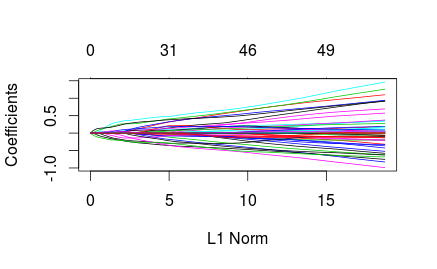
\includegraphics[]{Rplot1.png}
\center{\caption{Plot without cross-validation}}
\end{figure}
\begin{figure}[h]
\centering
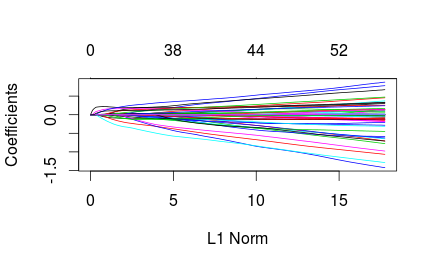
\includegraphics[]{Rplot2.png}
\center{\caption{Plot in conjunction with cross-validation}}
\end{figure}
The next steps deliver the sought mirs.
\begin{lstlisting}[style=base]
@> c = as.numeric(coef(out2)[-1])
> names(c) = colnames(X)
> idx = order(abs(c), decreasing=TRUE)
> c = c[idx,drop=FALSE]
> idx = abs(c) > 0
> data.frame(coef=c[idx])
                          coef
hsa-mir-874-3p   -1.584823e-01
hsa-mir-7-1-3p    1.032142e-01
hsa-mir-181c-3p  -6.623627e-02
hsa-mir-424-3p    6.393274e-02
hsa-mir-509-3-5p -2.417862e-02
hsa-mir-196b-5p   2.359241e-02
hsa-mir-92b-3p    6.039862e-05
\end{lstlisting}
According to the result, the selected mirs above affect the vital status most,
especially the mir "hsa-mir-874-3p". In spite of the relatively rough analysis
the result is still suitable as you can find information about some of the selected mirs
 in conjunction with ACC, especially the mir "hsa-mir-7-1-3p" or at least the mir-7
 microRNA precursor\footnote{\url{https://en.wikipedia.org/wiki/Mir-7_microRNA_precursor}}, 
seems to play a  role\footnote{\url{https://www.ncbi.nlm.nih.gov/pmc/articles/PMC4742203/}\\
 \url{https://www.google.com/patents/EP2657348A1?cl=en}}.


\section{Conclusion}
This technical report introduced the R package $EasyTCGA$  allowing easy and comfortable
 batch downloading of particular data types of TCGA from FireBrowse mentioned in the introduction. 
We presented all functions of the package and its applications. The package is quite easy to use, 
just some input parameters have to be specified, whereby almost all relevant input parameters are
listed or linked in the documentation or are provided by the package itself. \\
The drawback of the package is the low download speed depending on the data size of the data
query. Especially the download of all available specific data for a cohort can take some time. But 
this is primarily due to the Firebrowse API. Depending on the IPI it may occur that the output data frame is NULL
although the data for your query is available. You can prove it on FireBrowse\footnote{\url{http://firebrowse.org/}}.\\





\newpage
\section*{Acknowledgement}
\addcontentsline{toc}{section}{Acknowledgement}

This work has been supported by Deutsche Forschungsgemeinschaft
   (DFG) within the Collaborative Research Center SFB 876 "Providing
   Information by Resource-Constrained Analysis", project C1.








\end{document}